\section{Why a Virtual Observatory?}


\subsection{Interest of data in archives}
%%%%%%%---- BEGIN ----  ----%%%%%%
\begin{frame}
  \frametitle{Interest of data in archives}

  \begin{overlayarea}{\textwidth}{.6\textheight}
    \begin{onlyenv}<1>
      \hspace{0.15\hsize}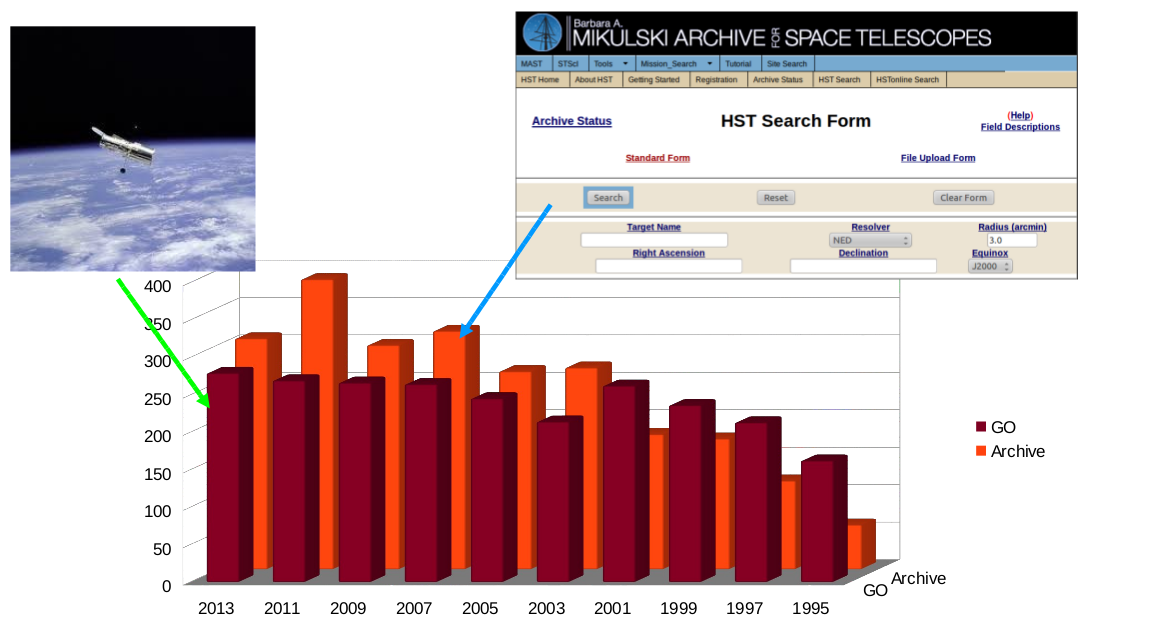
\includegraphics[width=0.7\textwidth]{hst-archive}%
      \src{Credits: E. Solano}
    \end{onlyenv}

    \begin{onlyenv}<2>
      \vspace{.5em}
      \hspace{0.1\hsize}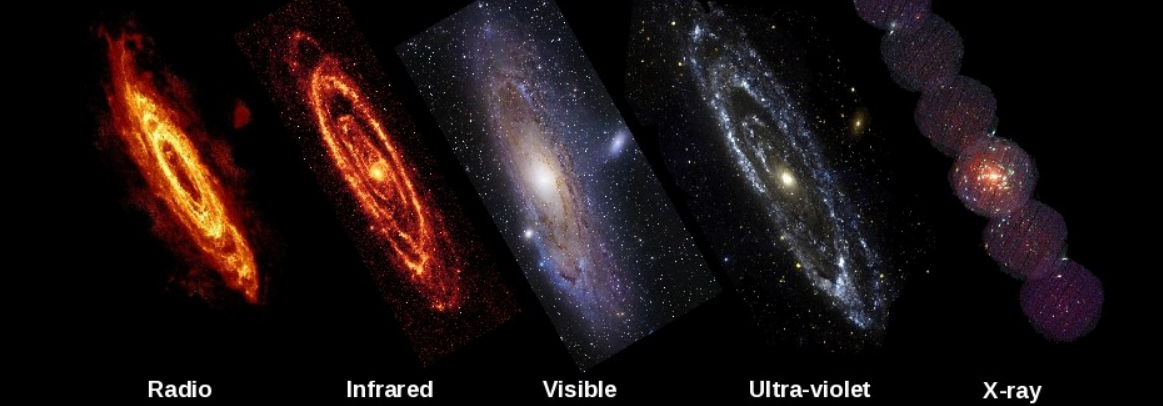
\includegraphics[width=0.8\textwidth]{multiwave}\\
      \src{M31 - ESA/NASA}
    \end{onlyenv}

    \begin{onlyenv}<3>
      \hspace{0.25\textwidth}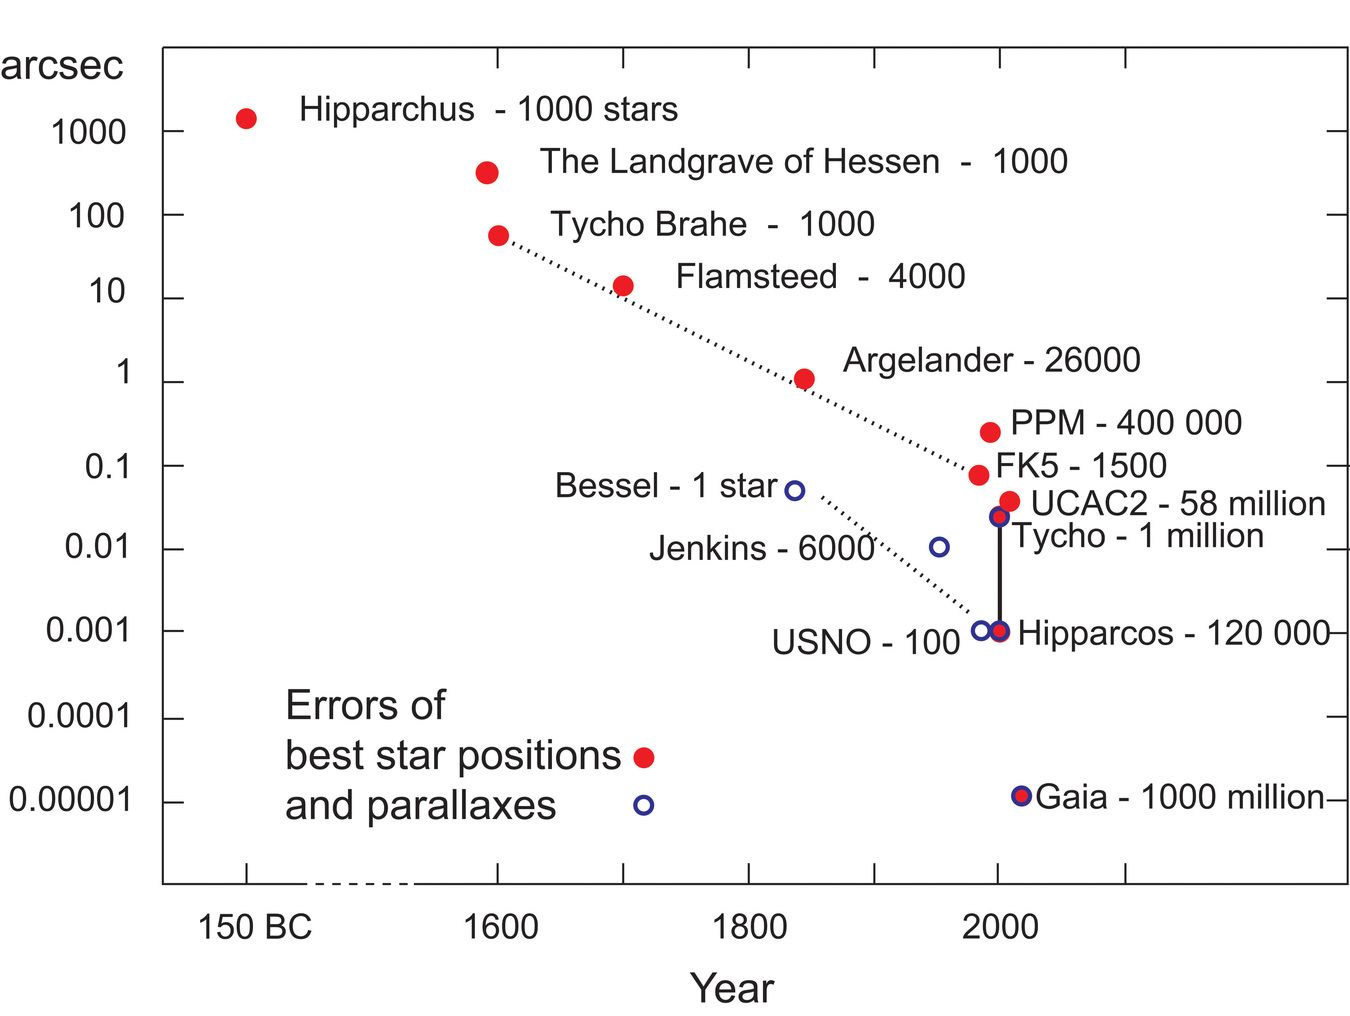
\includegraphics[width=.5\textwidth]{cata-acc}\\
      \vspace{-2.5em}
      \src{ESA}
    \end{onlyenv}

  \end{overlayarea}

  \begin{overlayarea}{\textwidth}{.3\textheight}
    \begin{columns}[T]

      \begin{column}{.35\textwidth}
        \begin{itemize}[<+->]
          \item \emph{Data from archives}
            \begin{itemize}[<.->]
              \item[$\circ$] Ever growing
              \item[$\circ$] Second life
              \item[$\circ$] \textbf{For other purposes}
            \end{itemize}
          \end{itemize}
      \end{column}


      \begin{column}{.35\textwidth}
        \begin{itemize}[<+->]
          \item \emph{Data complementarity}
            \begin{itemize}[<.->]
              \item[$\circ$] Multi-wavelength
              \item[$\circ$] Multi-resolution
              \item[$\circ$] Time-dependent
            \end{itemize}
          \end{itemize}
      \end{column}

      \begin{column}{.35\textwidth}
        \begin{itemize}[<+->]
          \item \emph{Data re-analysis}
            \begin{itemize}[<.->]
              \item[$\circ$] Astrometry
              \item[$\circ$] Photometry
              \item[$\circ$] Time-dependent
            \end{itemize}
          \end{itemize}
      \end{column}
  
    \end{columns}
  \end{overlayarea}

\end{frame}
%%%%%%%----  END  ----  ----%%%%%%





\subsection{The issues with archives}
%%%%%%%---- BEGIN ----  ----%%%%%%
\begin{frame}
  \frametitle{The issues with archives}

  \begin{columns}[T]

    \begin{column}{.5\textwidth}
      \begin{overlayarea}{\textwidth}{\textheight}

        \begin{onlyenv}<1>
          \vspace{1em}
          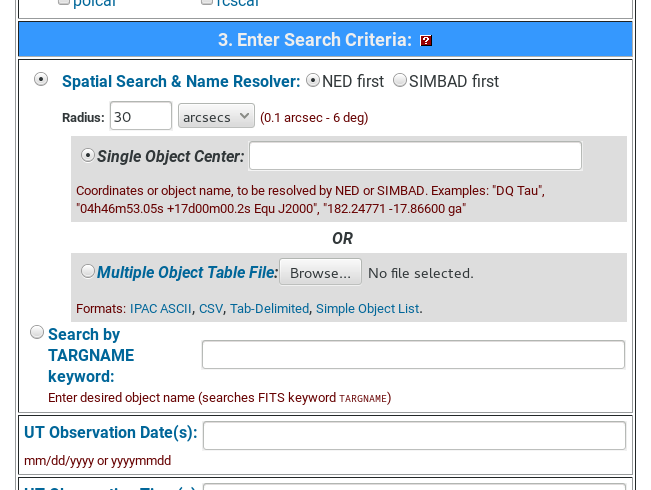
\includegraphics[width=\textwidth]{koa-target}\\
          \src{Keck archive query form}
        \end{onlyenv}
    
        \begin{onlyenv}<2>
          \vspace{2.5em}
          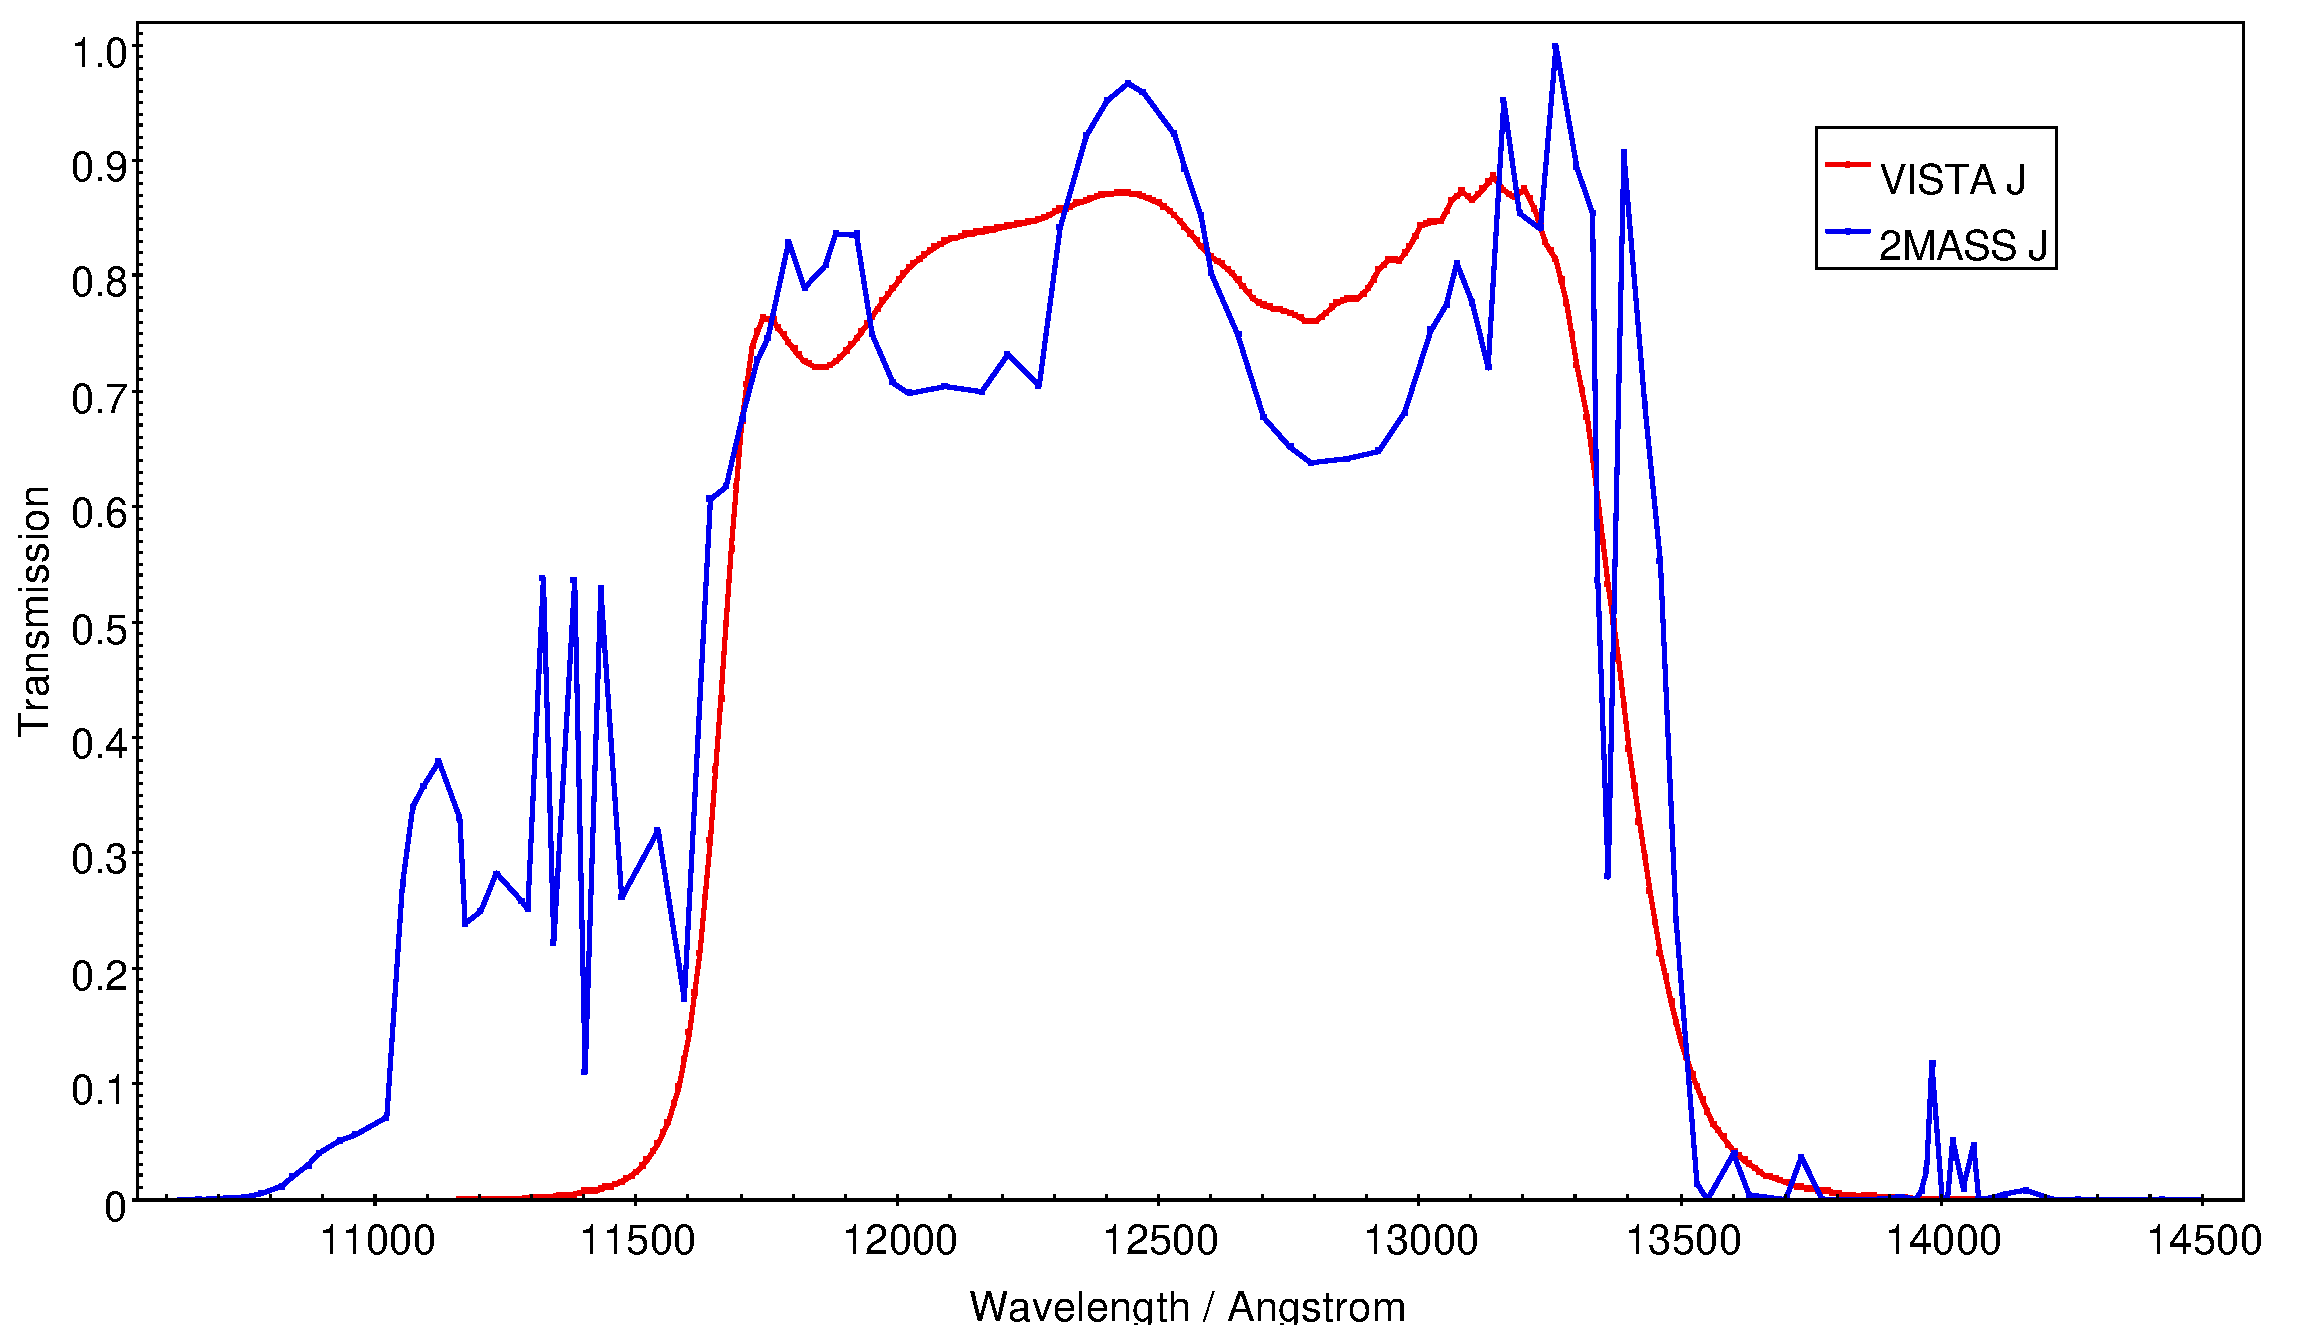
\includegraphics[width=\textwidth]{Jband}\\
          \src{Using SVO Filter service \& TOPCAT}
        \end{onlyenv}
    
        \begin{onlyenv}<3>
          \hspace{0.15\textwidth}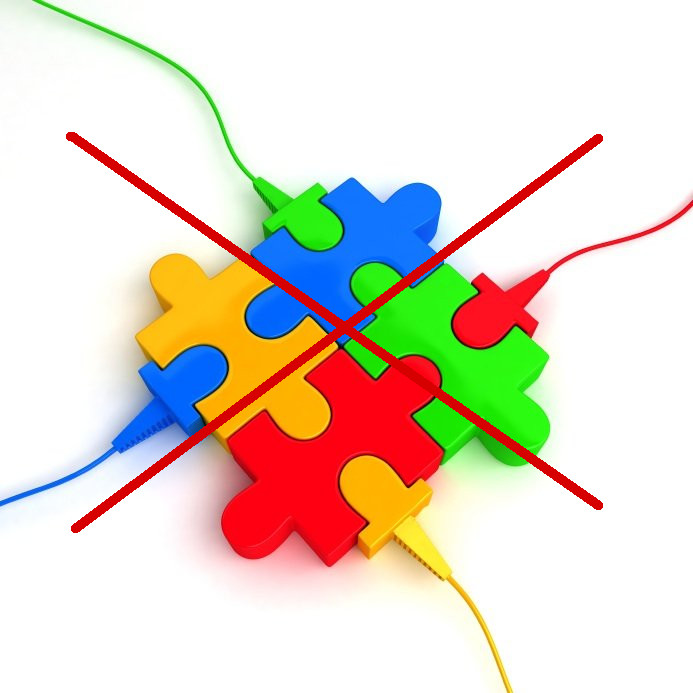
\includegraphics[width=0.7\textwidth]{plugpuzzle}\\
          \hspace{0.15\textwidth}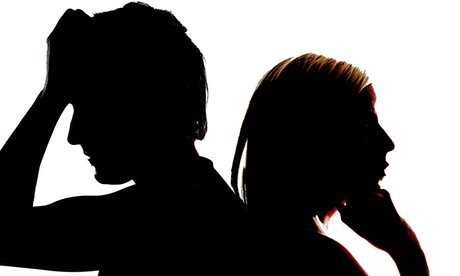
\includegraphics[width=0.7\textwidth]{too-hard}

        \end{onlyenv}

      \end{overlayarea}
    \end{column}

    \begin{column}{.6\textwidth}
      \begin{itemize}[<+->]
        \item \emph{Each archive has its standards}
          \begin{itemize}[<.->]
            \item[$\circ$] \textbf{Coordinates:} EQ, Ec, Gal
            \item[$\circ$] \textbf{Time:} TCB, OBT, TT
            \item[$\circ$] \textbf{I/O:} Target identifier
            \item[$\circ$] \textbf{I/O:} FITS, csv, ascii
          \end{itemize}

        \vspace{0.7em}
        \item \emph{Each instrument has its specifics}
          \begin{itemize}[<.->]
            \item[$\circ$] Filter transmission
            \item[$\circ$] Filter zeropoint
            \item[$\circ$] E.g.: 2MASS \textbf{vs} VISTA J?
          \end{itemize}

        \vspace{0.7em}
        \item[$\blacktriangleright$] \emph{Collect of information}
          \begin{itemize}[<.->]
            \item[$\circ$] Tedious task
            \item[$\circ$] Require multiple expertise
            \item[$\circ$] Tera $\rightarrow$ Peta $\rightarrow$ Zetabytes
            \item[$\circ$] Almost impossible
          \end{itemize}

        \end{itemize}
      \end{column}

  \end{columns}

\end{frame}
%%%%%%%----  END  ----  ----%%%%%%



\subsection{The Virtual Observatory}
%%%%%%%---- BEGIN ----  ----%%%%%%
\begin{frame}
  \frametitle{The Virtual Observatory}

  \begin{block}{Purpose of the Virtual Observatory}
    Provide an easy and efficient access to catalogs and data in
    astronomical archives, as well as analysis tools.
  \end{block}

  \vspace{2em}
  \hspace{0.25\textwidth}
\includegraphics[width=0.5\textwidth]{ivoa-members}


\end{frame}
%%%%%%%----  END  ----  ----%%%%%%
